\medskip
Durante a pesquisa de campo realizada com produtores de fazendas de 
\textit{Citrus reticulata} (mexerica), ambas localizadas no município de 
Pariquera-Açu, foram entrevistados os produtores identificados como Entrevistado 
A e Entrevistado B, os quais relataram experiências relevantes relacionadas ao 
manejo nutricional e fitossanitário em suas propriedades. 

\begin{figure}[H]
\centering
\caption{Entrevistado A  }%
\label{fig:Pesquisa-1}
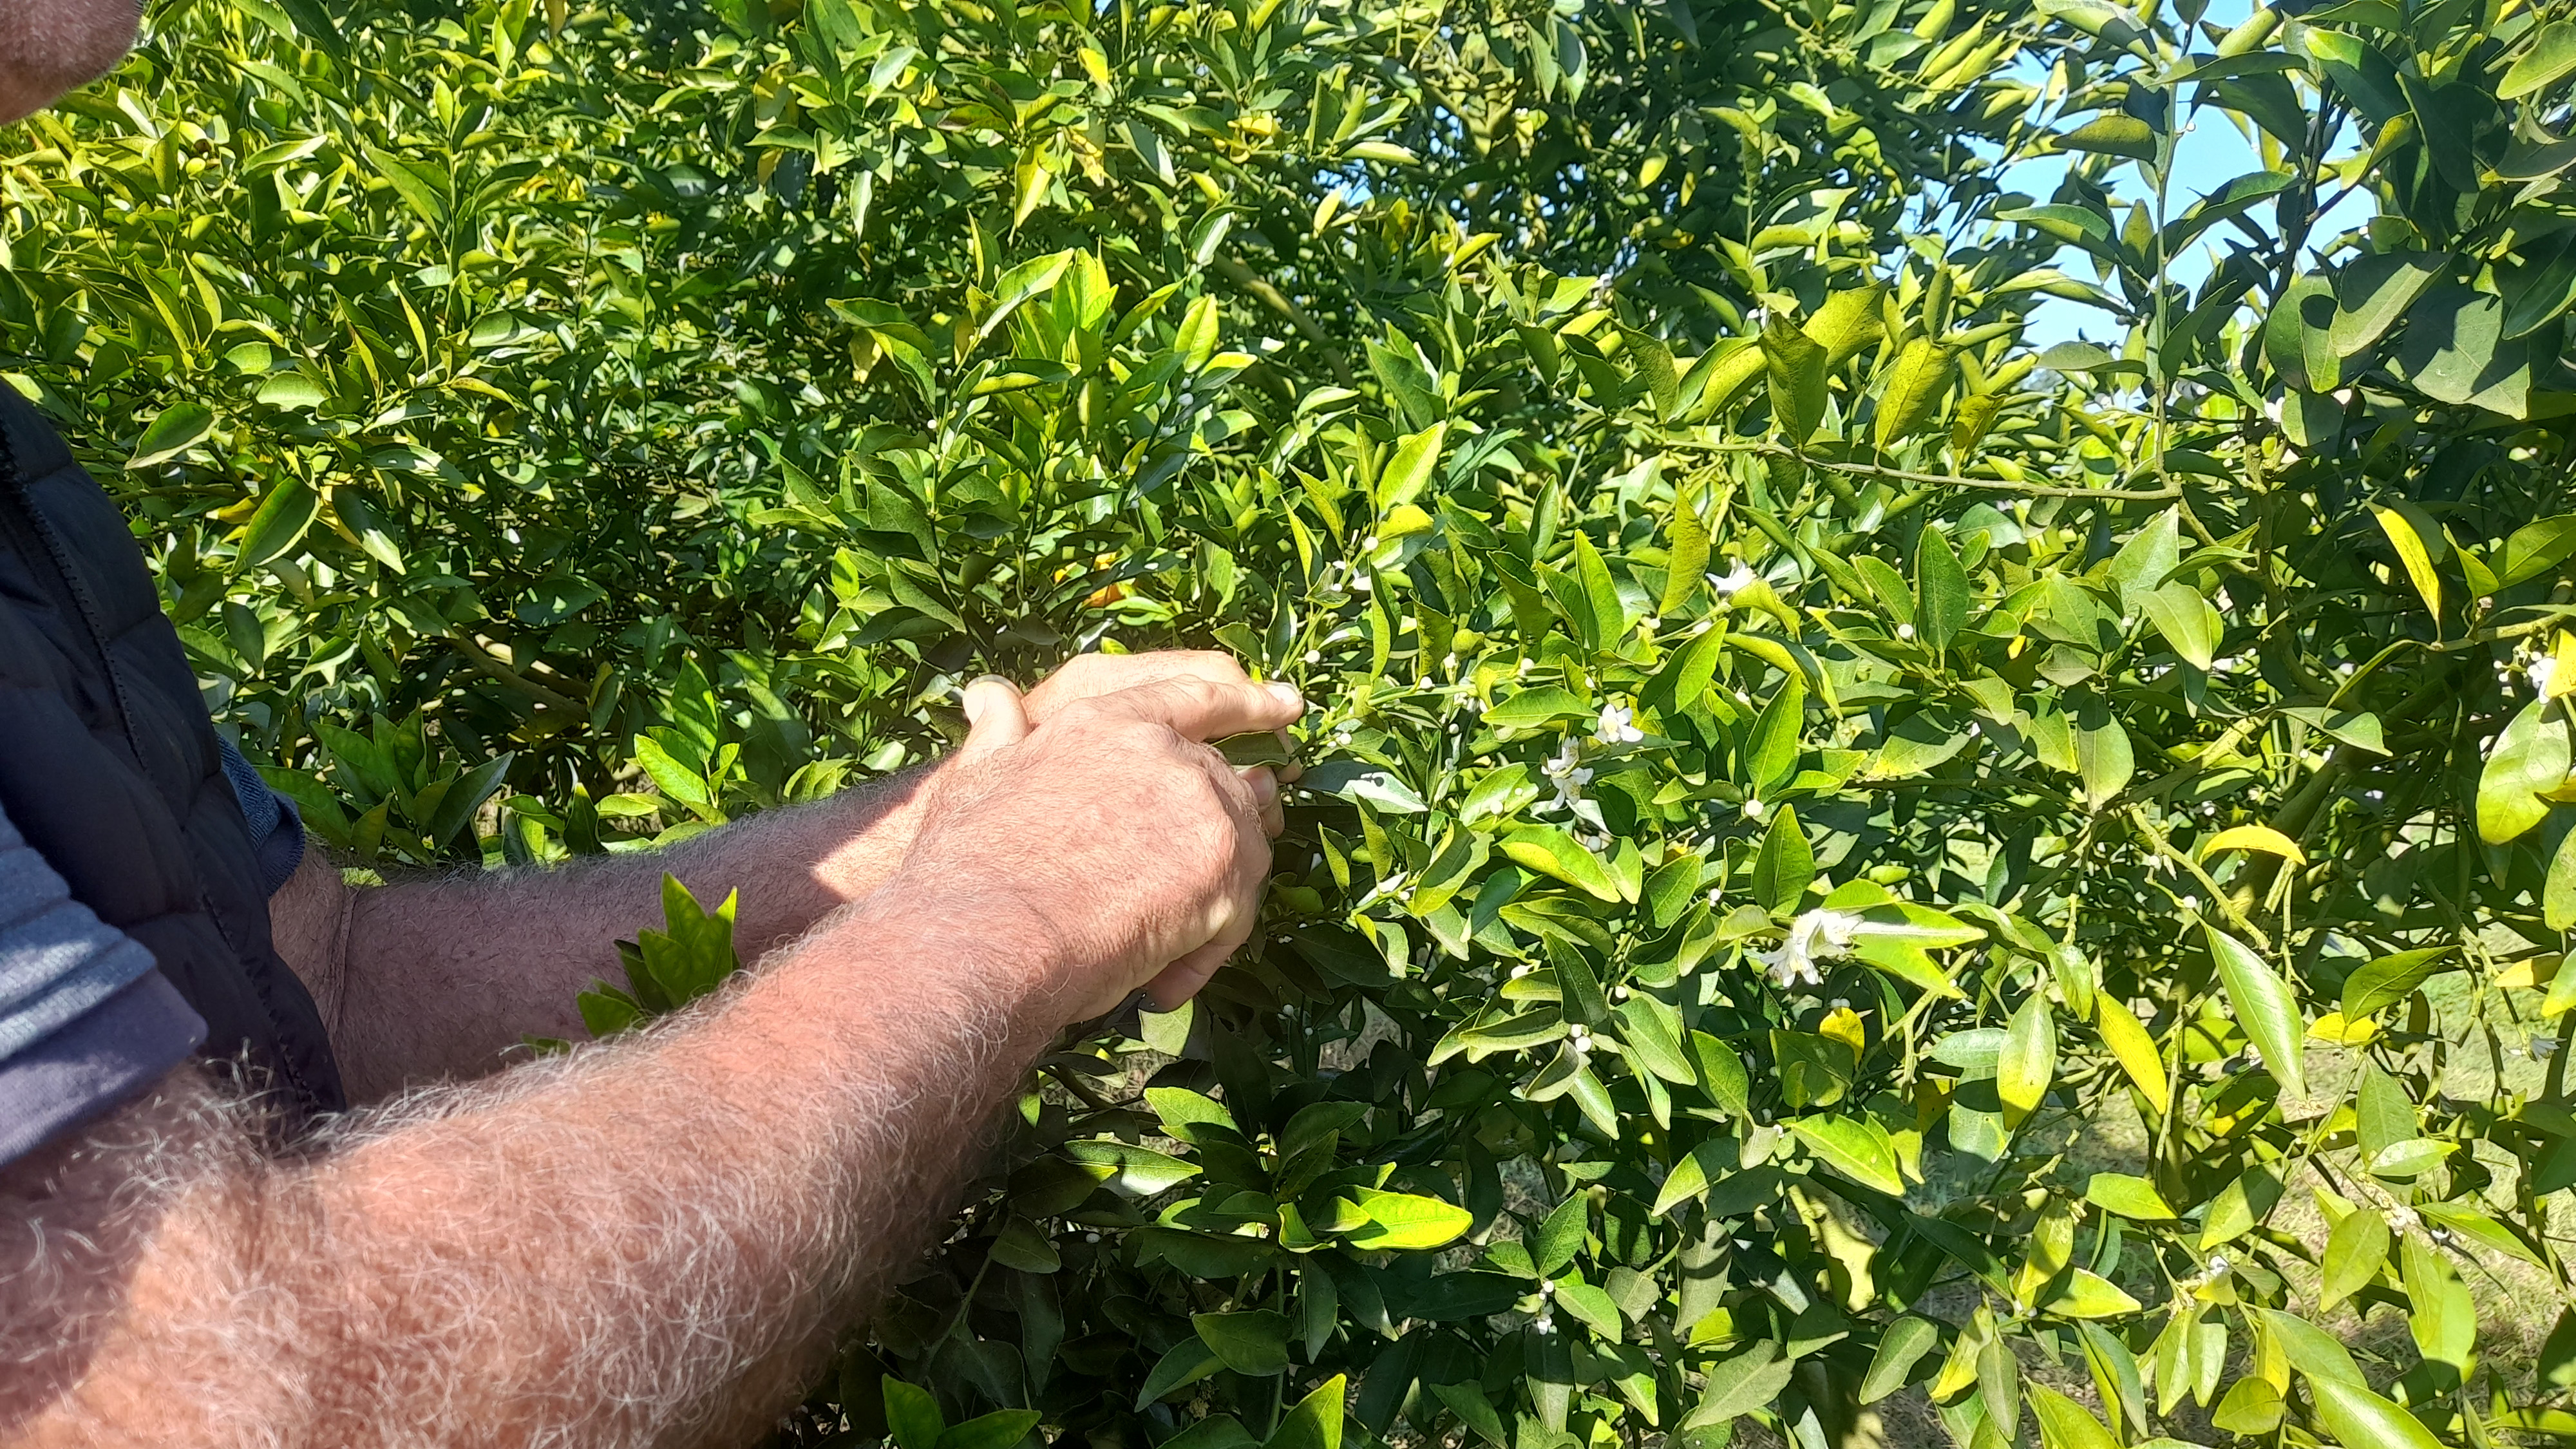
\includegraphics[width=0.8\textwidth]{Images/PesquisaCampo1.jpg}
\SourceOrNote{Equipe 21 - Vitalliz (2025)}
\end{figure}

\medskip
O Entrevistado A relatou que, em sua fazenda, já ocorreram deficiências de 
manganês e cobre nas plantas de \textit{Citrus reticulata} (mexerica). 
A suspeita surgiu devido ao amarelamento das folhas e à clorose internerval. 
A correção dessas deficiências foi realizada por meio da adubação com 
fertilizantes enriquecidos com os nutrientes necessários. O entrevistado 
afirmou conseguir distinguir alguns casos de deficiência de manganês e cobre 
e relatou já ter tido contato com a doença \textit{Greening}, identificada 
por sintomas como amarelamento e presença do \textit{Psilídeo}; nesses casos, 
houve perda total dos frutos. 

\medskip
Em sua fazenda, a falta de nutrientes é frequente, sendo o diagnóstico 
realizado por indicadores como amarelamento das folhas, frutos pequenos e 
produção reduzida. Mais da metade dos casos diagnosticados refere-se a deficiências 
nutricionais gerais. O entrevistado também destacou que um dos principais problemas 
enfrentados é o controle de pragas, e que, quando há algum problema na saúde das 
plantas, busca auxílio de técnico ou agrônomo. Além disso, realiza a verificação 
da saúde das plantas uma vez por mês. Ele e sua equipe contam com o auxílio de aplicativos 
e o apoio de especialistas para a verificação e controle das plantações. 

\begin{figure}[H]
\centering
\caption{Entrevistado A - Sinalização de árvore suspeita }%
\label{fig:Pesquisa-1}
\includegraphics[width=0.8\textwidth]{Images/PesquisaCampo2.jpg}
\SourceOrNote{Equipe 21 - Vitalliz (2025)}
\end{figure}

O Entrevistado A sinaliza árvores suspeitas utilizando uma fita. 
Essas plantas permanecem em observação para tratamento posterior, 
sob acompanhamento do técnico agrônomo.

\medskip
O Entrevistado B relatou ter enfrentado problemas de deficiência de manganês e cobre
em suas plantas, cuja identificação ocorreu por meio do diagnóstico realizado por um engenheiro 
agrônomo, que indicou as medidas corretivas. Em algumas ocasiões, esse profissional também 
realiza análise foliar. O entrevistado afirma conseguir distinguir as deficiências nutricionais 
da doença \textit{Greening} por meio da observação de sintomas, e relata já ter tido 
\textit{Greening} em sua fazenda. O diagnóstico baseia-se na experiência dos funcionários e 
na observação do estado da árvore e dos frutos, porém é tardio, pois as alterações nas folhas 
ocorrem somente em plantas já afetadas. Existem casos em que a planta continua produzindo frutos 
saudáveis mesmo estando doente; nesses casos, o pé não é cortado, apenas tratado, para evitar a 
disseminação da doença para outras plantas. Houve perda parcial da plantação devido ao 
\textit{Greening}, mas havia possibilidade de recuperação. Também são frequentes o amarelamento,
a perda e a diminuição dos frutos na fazenda. 

\medskip
O entrevistado afirma que a maioria dos casos de deficiência nutricional está relacionada
à falta de manganês. Os principais problemas enfrentados no cotidiano da plantação são a 
falta de conhecimento da maioria dos colaboradores para identificar problemas de saúde nas 
plantas de \textit{Citrus reticulata} (mexerica), o que se deve, em parte, ao predomínio do 
cultivo de banana na região, reduzindo o conhecimento específico sobre a cultura cítrica. 
Quando ocorre algum problema na plantação, é chamado um técnico para avaliar e corrigir 
eventuais problemas, como ácaros nos frutos, e as deficiências nutricionais acabam ficando 
em segundo plano. 

\medskip
O entrevistado realiza monitoramento da saúde das plantas em média uma vez por semana, 
geralmente por meio da observação dos funcionários durante o trabalho no pomar. 
Regularmente, não são utilizadas tecnologias para medir a saúde das plantas, mas, 
pontualmente, foram empregados adesivos amarelos para atrair insetos transmissores 
do \textit{Psilídeo}, drones para testar a aplicação de caldas e marcação com fita
plástica para monitorar plantas suspeitas de \textit{Greening}. 

\medskip
Diante das observações realizadas durante a pesquisa de campo, evidencia-se a 
importância deste estudo para a melhoria das práticas de manejo nutricional e 
fitossanitário nas plantações de \textit{Citrus reticulata} (mexerica). 
Verificou-se que o diagnóstico das deficiências nutricionais, especialmente 
de manganês e cobre, ainda ocorre de forma tardia e, em muitos casos, 
é confundido com sintomas da doença \textit{Greening}, resultando 
em perdas significativas na produção e no descarte de plantas potencialmente 
produtivas. O presente projeto propõe o desenvolvimento de um método de 
diagnóstico precoce das deficiências nutricionais por meio da análise foliar 
automatizada, reduzindo a necessidade de acompanhamento técnico constante e 
facilitando o monitoramento direto pelos produtores.
\medskip